\section{Pembagian bab}
Secara default pembagian bab pada latex menggunakan perintah \textit{section}, \textit{subsection}, \textit{subsubsection} dan \textit{subsubsubsection}. Untuk mengatur kedalaman suatu dokumen pada bab bab tertentu, kita dapat menggunakan perintah berikut ini pada bagian Preamble :



setcounter.secnumdepth


setcounter.tocdepth

Opsi yang digunakan pada syntax secnumdepth pada perintah verbcounter= seperti perintah diatas, berarti Anda telah merubah kedalaman bab yang Anda perbaharui sampai dengan level 5 yaitu section -- subsection -- subsubsection -- paragraph -- subparagraph. Sedangkan pada perintah dari opsi tocdepth berfungsi untuk membuat table of contents atau menampilkan kedalaman bab sampai dengan level 5, namun jika tidak di setel maka pada bagian level 3 kebawah tidak akan dapat ditampilkan pada bagian toc.


\section{Format Cetak}
Pada format LateX teks mempunyai bentuk plaintext, yang artinya teks tersebut belum diformat. Pada proses formatting teks dapat dilakukan dengan bahasa tersendiri yaitu bahasa markup. Hal paling mendasar antara lain cetak tebal, miring dan gari bawah. Cetak tebal menggunakan perintah \textit{textbf},cetak miring menggunakan perintah \textit{textit} dan garis bawah menggunakan perintah \textit{underline}.

\section{Tanda petik}
Tanda petik di Latex menggunakan petik miring dan petik satu. Petik miring biasanya berada pada sebelah angka satu di keyboard dan diakhiri petik satu. Ingat fungsi tanda petik hanya untuk melakukan quote atau pengutipan langsung. Untuk istilah bahasa inggris gunakan miring.

\begin{lstlisting}[caption=Contoh kalimat dalam tanda petik di Latex,label={lst:tandapetik}]
`kalimat dalam tanda petik'
\end{lstlisting}

\section{Penomoran}
Perintah penomoran pada latex biasanya menggunakan format \textit{Numbering} atau format \textit{Bullets}. Perintah yang digunakan pada format Numbering adalah \textit{enumerate} sedangkan untuk Bullets yang menyerupai poin menggunakan \textit{itemize}.
\par \textit{Numbering} merupakan perintah yang digunakan untuk membuat daftar berurut dengan penomoran menggunakan angka (numbered list), yang biasanya diberikan pada awal baris baru. Sedangkan \textit{Bullets} atau poin adalah perintah yang digunakan untuk membuat daftar berurut dengan penomoran berupa symbol atau poin (bulleted list).

\section{Karakter Khusus}
Untuk memberikan karakter khusus pada LaTex kita dapat menggunakan tanda \textit{backslash} didepan karakter yang ingin kita tandai. Terdapat beberapa karakter yang tidak bisa langsung digunakan seperti tanda \textit{ampersand}. Selain itu format pemberian kutipan pada LaTex berbeda dengan pemberian kutipan pada editor lainnya.
\par Format yang digunakan adalah tanda kutip 1 yang miring(`) sebagai tanda kutip pembuka dan tanda kutip 1 (') sebagai tanda penutup, jika format itu digunakan contohnya seperti ini : `quotes'.


\section{Kode Program}
Agar kita dapat memasukan kode program, kita dapat menggunakan perintah \textit{lstlisting}. Perintah ini  berfungsi untuk memasukkan atau menambahkan kode program apapun ke dalam file yang terpisah. Untuk memasukan perintah \textit{lstlisting} kita perlu menulis parameter \textit{caption} dan \textit{label} untuk memberikan penjelasan keterangan kode program dan sebagai sumber referensi dari label kode program.

\lstinputlisting[caption=Menambahkan kode program,label={lst:kodeprogram}]{src/1/lstlisting.tex}

\section{Menambahkan Gambar}
Cara menambahkan gambar seperti pada listing \ref{lst:kodegambar}.
\lstinputlisting[caption=Contoh kode untuk menambahkan gambar,label={lst:kodegambar}]{src/1/figure.tex}


\section{Tabel}
Untuk dapat membuat tabel kita harus menggunakan perintah \textit{table}. Selain itu kita juga perlu menambahkan referensi pada tabel yang terdapat dalam kalimat berdasarkan labelnya.
\lstinputlisting[caption=Menambahkan perintah table,label={lst:tabel}]{src/1/tabel.tex}

\section{Document class}

Pada dokumen Latex terdapat atau mempunyai beberapa struktur yang dicirikan dengan blok yang diberi apit oleh perintah begin dan end. Latex memberikan pilihan Class dokuman yang bisa di pakai, antara lain aadlah Book, Report, Article dan lain sebagainya. Class document book merupakan Class Document yang paling tepat untuk menulis, karena dapat mendukung table of contents yang dapat berfungsi langsung untuk generate daftar isi secara langsung.

Format ukuran font pada latex :

\begin{figure}[ht]
\centerline{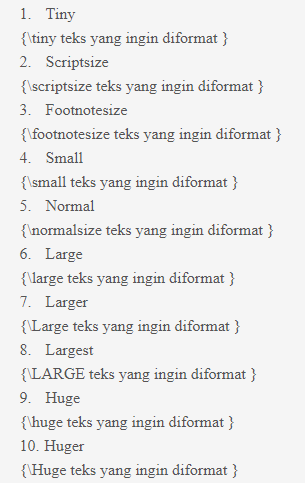
\includegraphics[width=0.7\textwidth]{figures/1.PNG}}
\caption{ukuran font}
\label{labelgambar1}
\end{figure}


\section{Costum Command}
Sesuai  dengan  namanya Costum Command, dimana ke unggulan latex ada fitur yang satu ini,
Pembuat dokumen ini dapat  membuat macro untuk kebutuhan yang sifatnya spesifik dan berulang-ulang,
dimana costum cummad dapat melakukan tanda bintang berjejer sebagai penanda garis.



